% Nome do capítulo
\chapter{Testes e Resultados}
% Label para referenciar
\label{cap5}

% Diminuir espaçamento entre título e texto
\vspace{-1.9cm}

% Texto do capítulo
%Para os testes foi simulado valores para cada um dos tipos de pés e pisadas. 

%\begin{figure}[H]
  % Alterar espaçamentos antes e depois do caption
%  \setlength{\abovecaptionskip}{0pt}
%  \setlength{\belowcaptionskip}{0pt}
%  % Caption
%  \caption[Pressão por sensor]{Pressão por sensor}
%  \centering
%  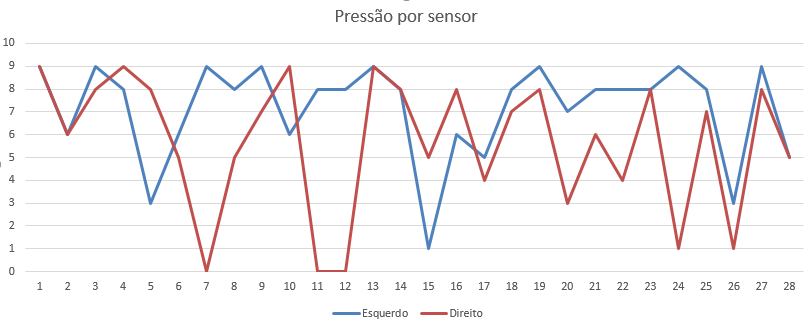
\includegraphics[width=.85\textwidth]{imagem/pressaoporsensor2.png}
  % Caption centralizada
%  \captionsetup{justification=centering}
%  \captionfont{\small{\textbf{\\Fonte: (DEVMEDIA, 2016) }}}	
%  \label{fig:UC}
%\end{figure}

%  Este documento foi compilado em ambiente linux (Ubuntu 10.04) usando o programa Kile - an Integrated LaTeX Environment - Version 2.0.85.
%  Para correta formatação os seguintes arquivos do pacote \textit{abntex} devem ser alterados.

 %   \begin{compactitem}
 %     \item[a)] Arquivo abnt.cls

%      No Ubuntu o arquivo fica armazenado em \textit{/usr/share/texmf/tex/latex/abntex}.
%      Comentar a linha 967: Linha comentada para reduzir o espaçamento entre o topo da página e o título.
 %     Alterar a linha 1143: Parâmetro alterado de 30pt para -30pt para reduzir o espaçamento entre o top da página e o título do apêndice.
%      Alterar a linha 985: Parâmetro alterado de 0pt para -30pt para reduzir o espaçamento entre o top da página e o título.
%      Alterar a linha 991: Parâmetro alterado de 45pt para 30pt para reduzir o espaçamento entre o texto e o título.

%      \item[b)] Arquivo acronym.sty

%      No Ubuntu o arquivo fica armazenado em \textit{/usr/share/texmf-texlive/tex/latex/acronym}.
 %     Alterar a linha 225: Inserir o separador -- entre acrônimo/descrição e remover o negrito com o \textit{normalfont}.
      %\item[\protect\AC@hypertarget{#1}{\acsfont{\normalfont{#2}}} --] #3 

 %   \end{compactitem}
 
% \begin{figure}[H]
  % Alterar espaçamentos antes e depois do caption
%  \setlength{\abovecaptionskip}{0pt}
%  \setlength{\belowcaptionskip}{0pt}
%  % Caption
%  \caption[Cronograma]{Cronograma}
%  \centering
%  \includegraphics[width=.99\textwidth]{imagem/Crono.png}
%  % Caption centralizada
%  \captionsetup{justification=centering}
%  \captionfont{\small{\textbf{\\Fonte: Elaborado pelo autor }}}	
%  \label{fig:UC}
%\end{figure}